\chapter{Benchmarks}\label{chapter:benchmarks}
In this chapter the SIDH implementations introduced in \autoref{chapter:existing_sidh} are compared with each other. For this purpose, a benchmarking suite was developed, which allows the generation of comparable benchmarks between these implementations. To get a better understanding of the results, the chapter starts with the tools and methodology used for benchmarking. The following implementations details provide precise internals of the benchmarking suite. This might be used for further development of the software. Finally, the benchmarking results are listed.
\section{Benchmarking Methodology}
In order to generate independent and stable benchmarking results, the benchmarking suite runs within a virtual environment: \textit{Docker} is used to separate the running suite from the host operating system. This reduces the influence of resource intensive processes, which might falsify benchmarking results. Moreover, \textit{Docker} enables a portable and scalable software solution.
\\
In the following, the process of benchmarking is described within five steps. In a short version, the required steps are:

\begin{enumerate}
  \item Create the benchmarking source code
  \item Compile the benchmarking source code
  \item Run \textit{Callgrind}
  \item Run \textit{Massif}
  \item Collect benchmarks
\end{enumerate}

\subsubsection{Create the benchmarking code}
Each software libraries presented in \autoref{chapter:existing_sidh} implements various cryptographic primitives. To avoid overhead when calculating benchmarks, only the required functions to generate a SIDH key exchange should be called. Thus, a simple benchmarking file is provided for each implementation, which calls the appropriate underlying API. This benchmarking file must ensure that all required headers are imported, the API is called correctly and a \texttt{main}-function is provided.

\subsubsection{Compile the benchmarking code}
Once the benchmarking source code is created, it needs to be compiled to a binary. Therefore, all required dependencies (libraries, headers, sourc code, ..) need to be provided to the compiler. The benchmarking suite provides a \texttt{Makefile} for each implementation, where the compilation process is implemented.
All compilations performed for the benchmarking suit must use consistent compiler optimizations. This ensures the comparability of the outputs. Currently, the optimization flag \texttt{-O3} is passed to the gcc compiler. Note, that CIRCL is implemented in GO and therefore the go compiler is used for compilation. Since this compiler does not provide optimization flags, the default compiler optimizations are used \parencite{gowiki2020compiler}.
To be able to extract benchmarks for specific functions \textit{inlining} is disabled during compilation. The C programming language offers the following directive to disable \textit{inlining} for a function:
\begin{lstlisting}[language=C]
// This function will not be inlined by the compiler
void __attribute__ ((noinline)) no_inlining() {
// ...
}

// This function might be inlined by the compiler
void inlining() {
// ...
}
\end{lstlisting}
The go compiler can be directly invoked with a no-inlining (\texttt{-l}) flag:
\begin{lstlisting}[language=Go]
go build -gcflags "-l"
\end{lstlisting}

\subsubsection{Run \textit{Callgrind}}
\textit{Callgrind} records function calls of a binary. For each call the executed instructions are counted. Moreover, the tool provides detailed information about the callee and how often functions are called.\textit{Callgrind} is part of \textit{Valgrind}, a profiling tool which allows deep analysis of executed binaries.\\
Callgrind is invoked on the command line via:
\begin{lstlisting}[language=Bash]
valgrind --tool=callgrind --callgrind-out-file=callgrind.out binary
\end{lstlisting}
The profiling data of callgrind is written to the file defined by \texttt{--callgrind-out-file}. This file might be analyzed using a graphical tool like \textit{KCachegrind} or any other analyzing script.
Running a binary using callgrind, slows down the execution times significantly. This is the main reason for the long execution times of the benchmarking suite. 

\subsubsection{Run \textit{Massif}}
\textit{Massif} measures memory usage of a binary, including heap and stack. \textit{Massif} is also part of the profiling tool \textit{Valgrind}. The tool creates multiple snapshots of the memory consumption during execution. Thus, one can extract the maximum memory consumption of a binary. The following command runs the \textit{Massif}:
\begin{lstlisting}[language=Bash]
valgrind --tool=massif --stacks=yes --massif-out-file=massif.out binary
\end{lstlisting}
The profiling data will be written to the file defined by \texttt{--massif-out-file}. \textit{Massif-visualizer} could be used to graphically analyze the data.

\subsubsection{Collect benchmarks}
Once the output files of \textit{Callgrind} and \textit{Massif} are produced, one can analyze the corresponding files to obtain:
\begin{enumerate}
\item Absolute instructions per function.
\item Maximum memory consumption during SIDH key exchange.
\end{enumerate}
This information is finally used by the benchmarking suite, to produce graphs and tables for further investigation.\\\\
To further increase the quality and reproducibility of the results, the cache of the virtual operating system is cleared, before \textit{Callgrind} and \textit{Massif} are executed. This is done via:
\begin{lstlisting}[language=Bash]
sync; sudo sh -c "echo 1 > /proc/sys/vm/drop_caches"
sync; sudo sh -c "echo 2 > /proc/sys/vm/drop_caches"
sync; sudo sh -c "echo 3 > /proc/sys/vm/drop_caches"
\end{lstlisting}


\section{Application Details}
The benchmarking suite is developed in Python3 on a Linux/Ubuntu operating system. Currently, the following implementations are included:
\begin{itemize}
\item SIKE working on: \texttt{p434, p503, p610, p751}
	\begin{itemize}
	\item Sike reference implementation (\texttt{SIKE\_Reference})
	\item Sike generic optimized implementation (\texttt{SIKE\_Generic})
	\item Sike generic optimized and compressed implementation (\texttt{SIKE\_Generic\_Compressed})
	\item Sike x64 optimized implementation (\texttt{SIKE\_x64})
	\item Sike x64 optimized and compressed implementation (\texttt{SIKE\_x64\_Compressed})
	\end{itemize}
\item PQCrypto-SIDH working on: \texttt{p434, p503, p610, p751}
	\begin{itemize}
	\item PQCrypto-SIDH generic optimized implementation (\texttt{Microsoft\_Generic})
	\item PQCrypto-SIDH generic optimized and compressed implementation \\ (\texttt{Microsoft\_Generic\_Compressed})
	\item PQCrypto-SIDH x64 optimized implementation (\texttt{Microsoft\_x64})
	\item PQCrypto-SIDH x64 optimized and compressed implementation \\ (\texttt{Microsoft\_x64\_Compressed})
	\end{itemize}
\item CIRCL working on: \texttt{p434, p503, p610, p751}
	\begin{itemize}
	\item CIRCL x64 optimized implementation (\texttt{CIRCL\_x64})
	\end{itemize}
\end{itemize}
Furthermore, the benchmarking suite provides classical elliptic curve Diffie-Hellman (ECDH) based on OpenSSL. Since SIDH is a candidate to replace current Diffie-Hellman algorithms, ECDH is intended as reference value: The objective is it to compare optimized modern ECDH with quantum-secure SIDH.\\
Since each parameter set of SIDH meet a different security level (compare \autoref{sidh_security}) ECDH is also instantiated with different curves, each matching a SIDH security level. The used elliptic curves are namely:
\begin{enumerate}
\item \texttt{secp256r1} (openssl: \texttt{prime256v1} \parencite{turner2009elliptic}): 128 bit security matching \texttt{SIKEp434} \parencite{brown2010sec}
\item \texttt{secp384r1} (openssl: \texttt{secp384r1}): 192 bit security matching \texttt{SIKEp610} \parencite{brown2010sec}
\item \texttt{secp512r1} (openssl: \texttt{secp521r1}): 256 bit security  matching \texttt{SIKEp751} \parencite{brown2010sec}
\end{enumerate}

\subsection{Application Flow}
This sections illustrates the application flow of the benchmarking suite (see \autoref{fig:app_flow}). Once triggered to run benchmarks, the following procedure is repeated for every implementation: The suite first compiles the benchmarking code. The binary is then executed multiple times via \textit{Callgrind} and \textit{Massif} to generate multiple benchmark measurements. 
\\
Finally, the results are visualized in different formats. Graphs compare the recorded instruction counts and the peak memory consumption among implementations instantiated with comparable security classes. A HTML table lists detailed benchmarks and the Latex output is used for this document.

\begin{figure}[H]
  \centering
  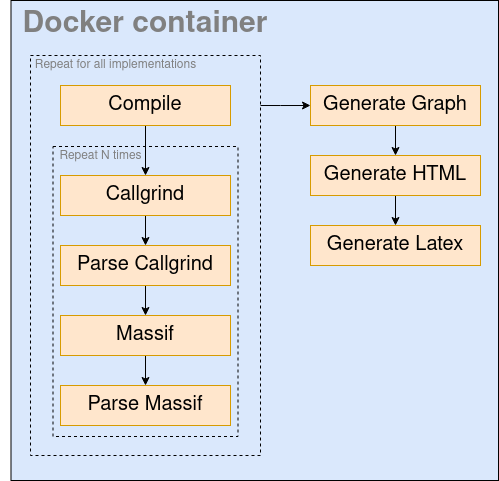
\includegraphics[width=0.8\textwidth]{benchmarks/application_flow}
  \caption[Flow chart of the benchmarking suite.]
  {Flow chart of the benchmarking suite. For each SIDH implementation, the source code is compiled and benchmarked multiple times. The benchmarking results are visualized in different format: Graphs, HTML and Latex.
  } \label{fig:app_flow}
\end{figure}




\subsection{Application Structure}
\subsection{Adding Implementations}
\section{Usage}
\section{Results}